\section{Tvorba a rozšiřování schémat XSD}
% Jaká aplikační schémata pro BU jsou implementovaná do XSD 

\begin{frame}
\frametitle{Aplikační schémata tématu Budovy}
\begin{center}
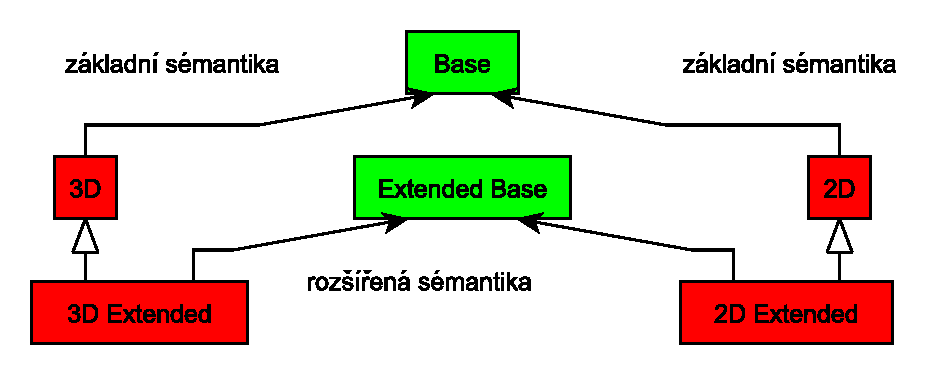
\includegraphics[scale=0.7]{obrazky/BU_schemas.pdf}
\end{center}
\end{frame}

\begin{frame}
\frametitle{Možnosti implementace aplikačních schémat}
\begin{center}
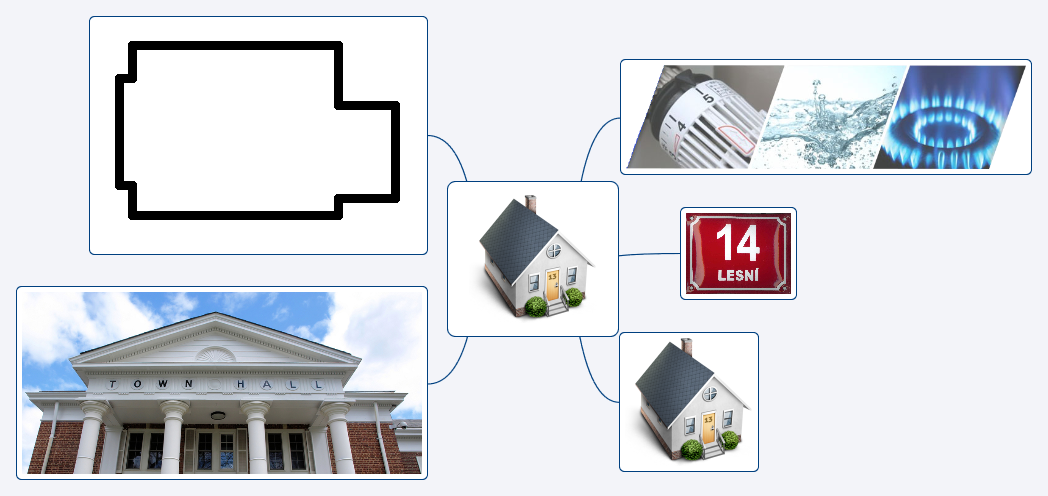
\includegraphics[scale=0.3]{obrazky/connection.png}
\end{center}
\end{frame}

\begin{frame}
\frametitle{Tvorba XSD -- základ}
\begin{center}
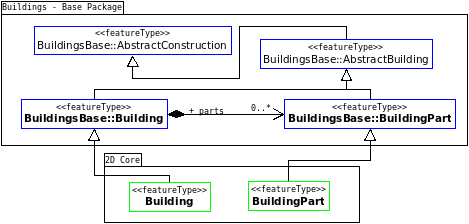
\includegraphics[scale=0.65]{obrazky/BuildingsBase2D.png}
\end{center}
\end{frame}

\begin{frame}
\frametitle{Tvorba XSD -- dědičnost}
\begin{center}
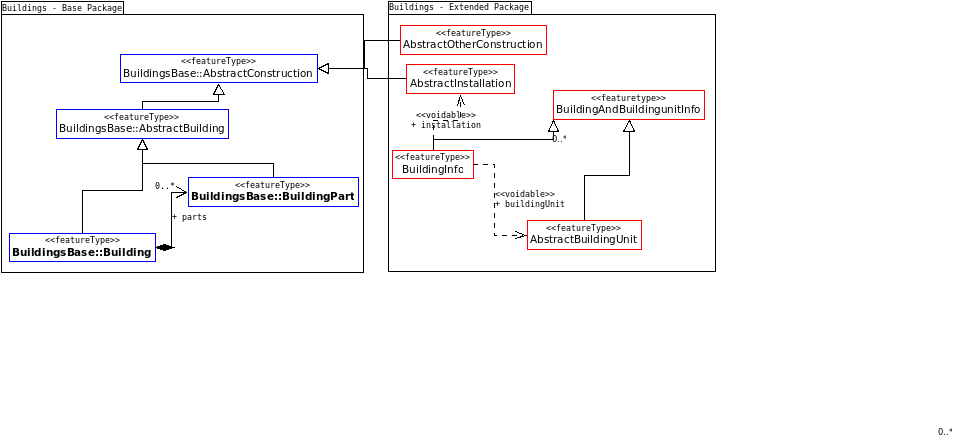
\includegraphics[scale=0.45]{obrazky/BU_ExtDedicnost.png}
\end{center}
\end{frame}

\begin{frame}
\frametitle{Tvorba XSD -- dědičnost}
\begin{center}
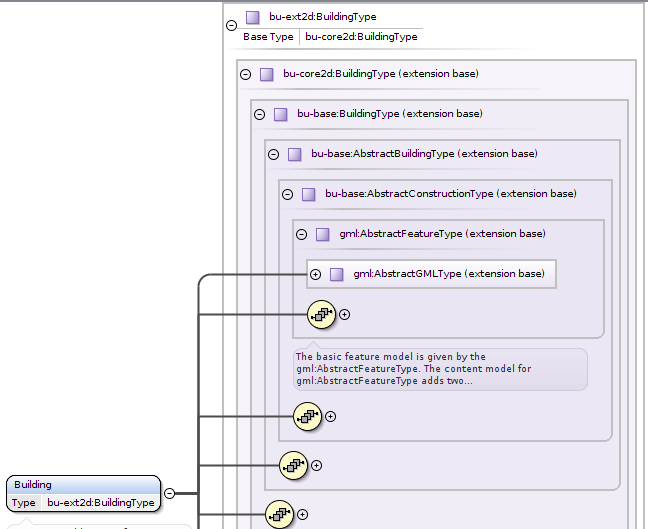
\includegraphics[scale=0.35]{obrazky/BU_oXygen.png}
\end{center}
\end{frame}

\begin{frame}
\frametitle{Tvorba XSD -- geometrie}
\begin{center}
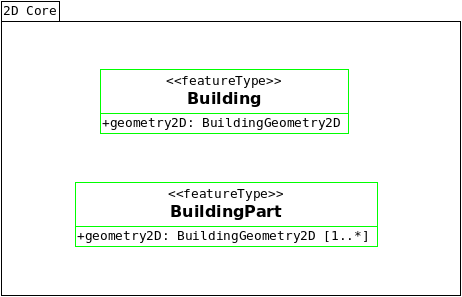
\includegraphics[scale=0.45]{obrazky/geometrie.png}
\end{center}
\end{frame}

\begin{frame}
\frametitle{Tvorba XSD -- vícenásobná dědičnost}
\begin{center}
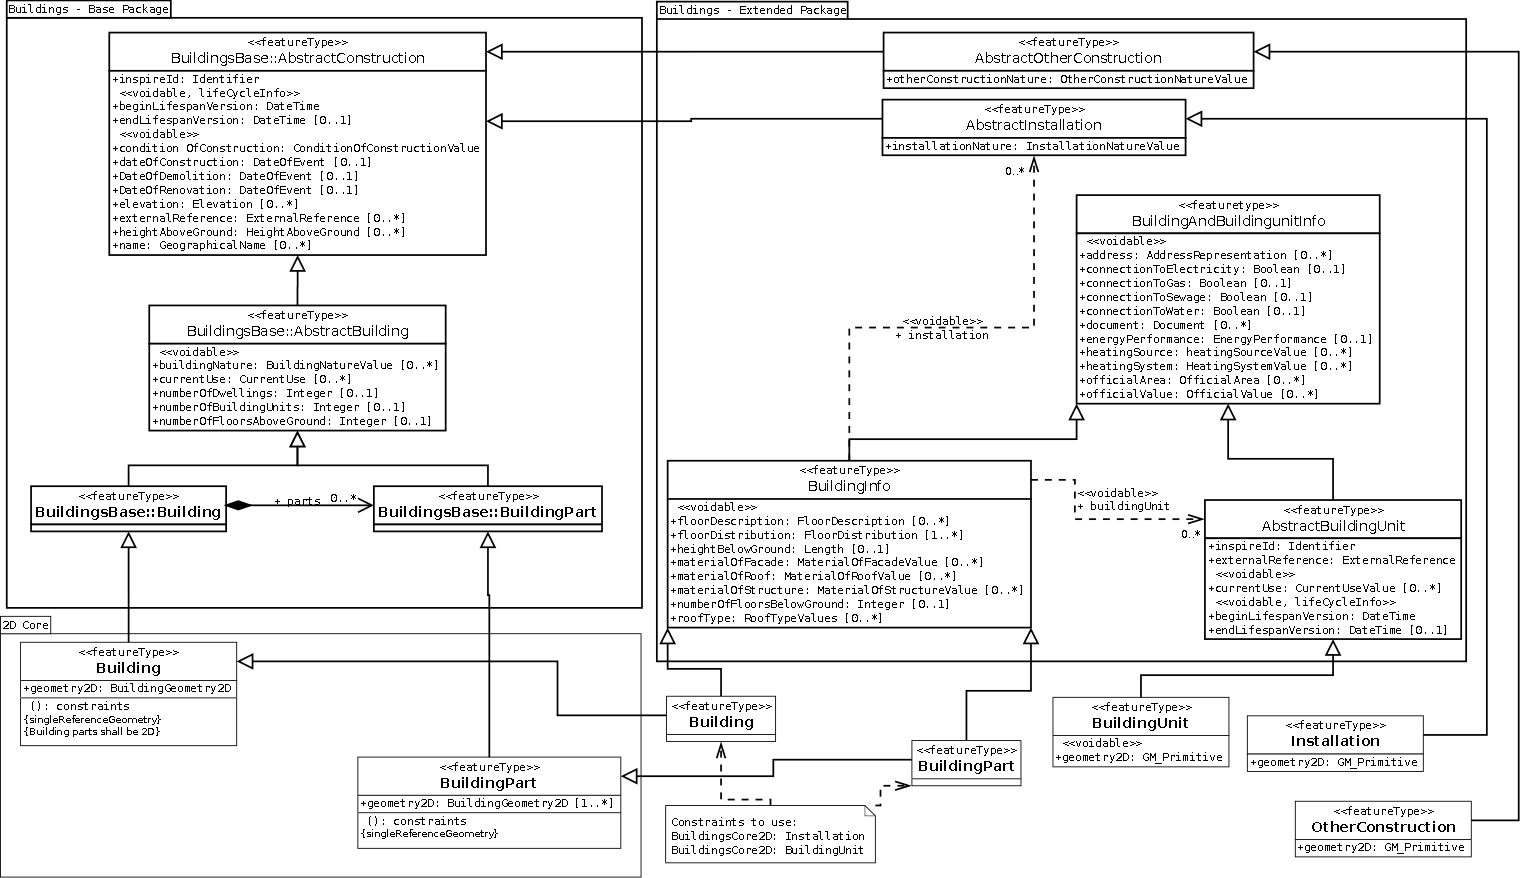
\includegraphics[scale=0.15]{obrazky/BuildingsExtended2D.png}
\end{center}
\end{frame}

\begin{frame}
\frametitle{Tvorba XSD -- vícenásobná dědičnosti}
\begin{center}
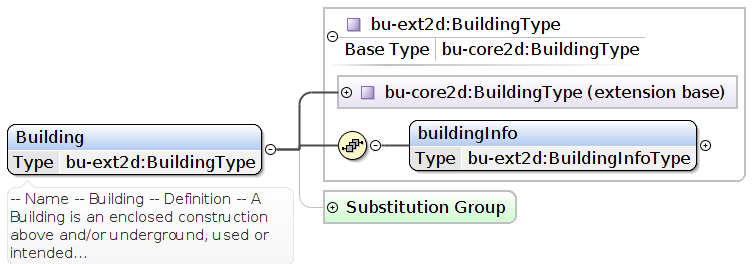
\includegraphics[scale=0.4]{obrazky/BU_dedicnost_info.png}
\end{center}
\end{frame}

\begin{frame}
\frametitle{Nová schémata XSD}
\begin{itemize}
\item \url{http://services.cuzk.cz/xsd/inspire/bu-ext2d/3.0/BuildingsExtended2D.xsd}
\item \url{http://services.cuzk.cz/xsd/inspire/bu-ext/3.0/BuildingsExtendedBase.xsd}
\end{itemize}
\end{frame}

